
\section{Preliminaries}
\label{sec:preliminaries}

Sequence data structures considered in this paper (for collaborative editing)
belong to the optimistic class of replication~\cite{saito2005optimistic}. Each
replica owner (a collaborator) directly performs operations on its local copy
and informs the other owners by broadcasting these operations. The consistency
criteria ensured by such optimistic replication is called strong eventual
consistency~\cite{shapiro2011comprehensive} upon the assumption of the eventual
delivery of operations, i.e., they guarantee that all replicas will eventually
converge to an identical state when the system becomes quiescent. This
consistency criterion is weaker than sequential consistency and linearisability
and is not comparable with causal consistency, yet strong enough for
collaborative edition~\cite{shapiro2011comprehensive}.

Sequence replicated data structures (\emph{sequence} for short) are the closest
structures that can implement a shared document. A sequence provides two
commutative operations: insert and delete. Operations can be integrated in any
order as soon as the deletion of an element follows its insertion.

The sequence is composed of elements and a unique and immutable identifier is
associated with each of these elements. The sequence can be seen as a set of
pairs $\langle element, identifier \rangle$. A total order is assumed on
identifiers and this order relation allows seeing the set of pairs as a
sequence. The projection of a sequence on the elements builds the document.

When a collaborator performs an insert operation, it first allocates the
identifier of the element to insert. For instance, let us consider a sequence
QWTY with the unique, immutable, and totally ordered integer identifiers $1$,
$2$, $4$, $8$ respectively. A collaborator inserts the element E between W
and T. The natural identifier that comes to mind is $3$. The resulting
sequence is QWETY. However, R cannot be inserted between E and T since
$3$ and $4$ are contiguous. The space of identifiers must be enlarged to handle
the new insertion. If we consider identifiers as decimal numbers, $3.1$ can be
associated with the character R. If a new character has to be inserted
between E and R, a new identifier will be allocated between $3$ and
$3.1$. Again, the space will be extended resulting in a new identifier $3.0$
suffixed by any non null integer. Let $X$ be the suffix, the order is preserved
since $(3 < 3.0.X < 3.1)$.

Such growing identifiers are called variable-size identifiers. The main
objective is to keep the growth of the size of the identifiers under a sublinear
boundary.

\subsection{Variable-size Identifiers}
\label{subsec:variable}

Variable-size identifiers can be represented as a concatenation of basic
elements (e.g. integers). The resulting sequence can be represented by a tree
structure where the elements of the sequence are stored at the nodes and where
the edges of the tree are labelled such that a path from the root to a node
represents the identifier of the element stored at this node. For instance, the
character $R$ in the previous example is accessible following the path composed
of the edges labelled $3$ then $1$. More formally, a sequence is a tree where
each node contains a value i.e. an element of the sequence (over an alphabet
$\mathcal{A}$). The tree is a set of pairs
$\langle\mathcal{P}\subset\{\mathbb{N}\}^*,\, \mathcal{A} \rangle$, i.e., each
element has a path. Additionally, a total order
($\mathcal{P}$,$<_{\mathcal{P}}$) provides an ordering among the paths which
allows to retrieve the order of the elements in the sequence. Notation: a path
composed of $e$ edges labelled $\ell_1,\ell_2,\ldots,\ell_e$ will be noted
$[\ell_1.\ell_2\ldots\ell_e]$.

\begin{figure*}
  \centering
  \subfloat[The tree is the unions of identifiers.]
  [\label{fig:treemodelexample}The tree representing the sequence is
  built by the union of identifiers and mainly uses paths to order its
  characters.]
  {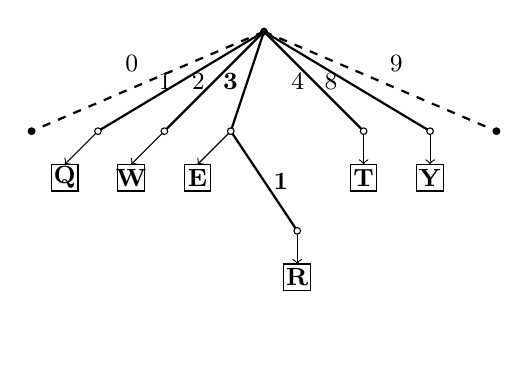
\begin{tikzpicture}[scale=1.2]

\newcommand\Y{-30};
\newcommand\ADDY{-10};

  %% node to node
  \small
  \draw[dashed,thick] (0pt,0pt) -- node[anchor=south east]{0} (-70pt,-30pt);
  \draw[thick] (0pt,0pt) -- node[anchor=east]{1} (-50pt,-30pt); %% Q
  \draw[thick] (0pt,0pt) -- node[anchor=east]{2} (-30pt,-30pt); %% W
  \draw[thick] (0pt,0pt) -- node[anchor=east]{\textbf{3}} (-10pt,-30pt); %% E
  \draw[thick] (0pt,0pt) -- node[anchor=east]{4} ( 30pt,-30pt); %% T
  \draw[thick] (0pt,0pt) -- node[anchor=east]{8} ( 50pt,-30pt); %% Y
  \draw[dashed,thick] (0pt,0pt) -- node[anchor=south west]{9} ( 70pt,-30pt);

  \draw[thick] (-10pt,-30pt) -- node[anchor=west]{\textbf{1}} ( 10pt,-60pt); %% R
%  \draw[thick] (-10pt,-30pt) -- node[anchor=west]{\textbf{0}} (-10pt,-60pt);
%  \draw[thick] (-10pt,-60pt) -- node[anchor=east]{\textbf{X}} (  0pt,-90pt); %% ?


  %% node to element
  \draw[->] (-50pt,\Y pt) -- (-60pt, \ADDY +\Y pt);
  \draw[->] (-30pt,\Y pt) -- (-40pt, \ADDY +\Y pt);
  \draw[->] (-10pt,\Y pt) -- (-20pt, \ADDY +\Y pt);
  \draw[->] ( 30pt,\Y pt) -- ( 30pt, \ADDY +\Y pt);
  \draw[->] ( 50pt,\Y pt) -- ( 50pt, \ADDY +\Y pt);

  \draw[->] ( 10pt,2 * \Y pt) -- ( 10pt, \ADDY + 2 * \Y pt);
%  \draw[->] (  0pt,3 * \Y pt) -- (  0pt, \ADDY + 3 * \Y pt);

  %% nodes
  \draw[fill=black] ( 0pt,  0pt) circle (1pt); 
  \draw[fill=black] (-70pt, -30pt) circle (1pt); 
  \draw[fill=white] (-50pt, -30pt) circle (1pt); %% Q
  \draw[fill=white] (-30pt, -30pt) circle (1pt); %% W
  \draw[fill=white] (-10pt, -30pt) circle (1pt); %% E
  \draw[fill=white] ( 30pt, -30pt) circle (1pt); %% T
  \draw[fill=white] ( 50pt, -30pt) circle (1pt); %% Y
  \draw[fill=black] ( 70pt, -30pt) circle (1pt);

%  \draw[fill=white] (-10pt, 2 * \Y pt) circle (1pt); %% R
  \draw[fill=white] ( 10pt, 2 * \Y pt) circle (1pt); %% x
%  \draw[fill=white] (  0pt, 3 * \Y pt) circle (1pt); %% ?

  %% elements
  \draw[fill=white](-60pt,-4 + \ADDY + \Y pt)
  node{\textbf{Q}} +(-4pt,-4pt) rectangle +(4pt,4pt) ; %% Q
  \draw[fill=white](-40pt,-4 + \ADDY + \Y pt)
  node{\textbf{W}} +(-4pt,-4pt) rectangle +(4pt,4pt) ; %% W
  \draw[fill=white](-20pt,-4 + \ADDY + \Y pt)
  node{\textbf{E}} +(-4pt,-4pt) rectangle +(4pt,4pt) ; %% E
  \draw[fill=white]( 30pt,-4 + \ADDY + \Y pt)
  node{\textbf{T}} +(-4pt,-4pt) rectangle +(4pt,4pt) ; %% T
  \draw[fill=white]( 50pt,-4 + \ADDY + \Y pt)
  node{\textbf{Y}} +(-4pt,-4pt) rectangle +(4pt,4pt) ; %% Y

  \draw[fill=white]( 10pt,-4 + \ADDY + 2 * \Y pt)
  node{\textbf{R}} +(-4pt,-4pt) rectangle +(4pt,4pt) ; %% R
%  \draw[fill=white](  0pt,-4 + \ADDY + 3 * \Y pt)
%  node{\textbf{?}} +(-4pt,-4pt) rectangle +(4pt,4pt) ; %% ?
  \draw(0, -8+\ADDY+ 2.5*\Y pt);

\end{tikzpicture}
}
  \hspace{20pt}
  \subfloat[Disambiguators operate when same paths have been allocated.]
  [\label{fig:disexample}The tree uses disambiguators to maintain an
  equivalent state, even in presence of concurrent operations resulting
  in same paths.]
  {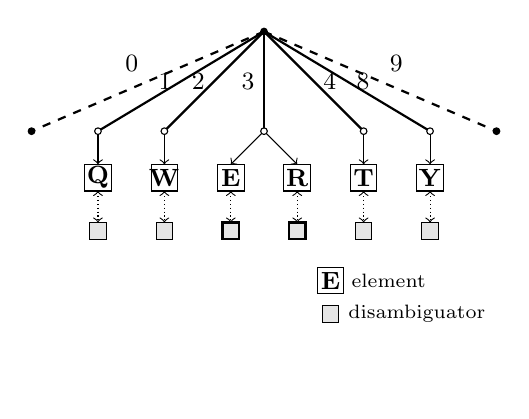
\begin{tikzpicture}[scale=1.2]

\newcommand\Y{-30};
\newcommand\ADDY{-10};

  %% node to node
  \small
  \draw[dashed,thick] (0pt,0pt) -- node[anchor=south east]{0} (-70pt,\Y pt);
  \draw[thick] (0pt,0pt) -- node[anchor=east]{1} (-50pt, \Y pt); %% Q
  \draw[thick] (0pt,0pt) -- node[anchor=east]{2} (-30pt, \Y pt); %% W
  \draw[thick] (0pt,0pt) -- node[anchor=east]{3} (  0pt, \Y pt); %% E R
  \draw[thick] (0pt,0pt) -- node[anchor=west]{4} ( 30pt, \Y pt); %% T
  \draw[thick] (0pt,0pt) -- node[anchor=west]{8} ( 50pt, \Y pt); %% Y
  \draw[dashed,thick] (0pt,0pt) -- node[anchor=south west]{9} ( 70pt, \Y pt);

  %% node to element
  \draw[->] (-50pt,\Y pt) -- (-50pt, \ADDY +\Y pt);
  \draw[->] (-30pt,\Y pt) -- (-30pt, \ADDY +\Y pt);
  \draw[->] (  0pt,\Y pt) -- (-10pt, \ADDY +\Y pt);
  \draw[->] (  0pt,\Y pt) -- ( 10pt, \ADDY +\Y pt);
  \draw[->] ( 30pt,\Y pt) -- ( 30pt, \ADDY +\Y pt);
  \draw[->] ( 50pt,\Y pt) -- ( 50pt, \ADDY +\Y pt);

  %% element to desambiguator
  \draw[<->,densely dotted](-50pt,-8+\ADDY + \Y pt)--(-50pt,2.75*\ADDY+\Y pt);
  \draw[<->,densely dotted](-30pt,-8+\ADDY + \Y pt)--(-30pt,2.75*\ADDY+\Y pt);
  \draw[<->,densely dotted](-10pt,-8+\ADDY + \Y pt)--(-10pt,2.75*\ADDY+\Y pt);
  \draw[<->,densely dotted]( 10pt,-8+\ADDY + \Y pt)--( 10pt,2.75*\ADDY+\Y pt);
  \draw[<->,densely dotted]( 30pt,-8+\ADDY + \Y pt)--( 30pt,2.75*\ADDY+\Y pt);
  \draw[<->,densely dotted]( 50pt,-8+\ADDY + \Y pt)--( 50pt,2.75*\ADDY+\Y pt);

  %% nodes
  \draw[fill=black] ( 0pt, 0 pt) circle (1pt); 
  \draw[fill=black] (-70pt, \Y pt) circle (1pt); 
  \draw[fill=white] (-50pt, \Y pt) circle (1pt); %% Q
  \draw[fill=white] (-30pt, \Y pt) circle (1pt); %% W
  \draw[fill=white] (  0pt, \Y pt) circle (1pt); %% E
  \draw[fill=white] ( 30pt, \Y pt) circle (1pt); %% T
  \draw[fill=white] ( 50pt, \Y pt) circle (1pt); %% Y
  \draw[fill=black] ( 70pt, \Y pt) circle (1pt);

  %% desambiguator
  \draw[fill=gray!20] (-50pt,-2.5+2.75*\ADDY+\Y pt)
  +(-2.5pt,-2.5pt) rectangle +(2.5pt,2.5pt);
  \draw[fill=gray!20] (-30pt,-2.5+2.75*\ADDY+\Y pt)
  +(-2.5pt,-2.5pt) rectangle +(2.5pt,2.5pt);
  \draw[fill=gray!20, thick] (-10pt,-2.5+2.75*\ADDY+\Y pt)
  +(-2.5pt,-2.5pt) rectangle +(2.5pt,2.5pt);
  \draw[fill=gray!20, thick] ( 10pt,-2.5+2.75*\ADDY+\Y pt)
  +(-2.5pt,-2.5pt) rectangle +(2.5pt,2.5pt);
  \draw[fill=gray!20] ( 30pt,-2.5+2.75*\ADDY+\Y pt)
  +(-2.5pt,-2.5pt) rectangle +(2.5pt,2.5pt);
  \draw[fill=gray!20] ( 50pt,-2.5+2.75*\ADDY+\Y pt)
  +(-2.5pt,-2.5pt) rectangle +(2.5pt,2.5pt);

  %% elements
  \draw[fill=white](-50pt,-4 + \ADDY + \Y pt)
  node{\textbf{Q}} +(-4pt,-4pt) rectangle +(4pt,4pt) ; %% Q
  \draw[fill=white](-30pt,-4 + \ADDY + \Y pt)
  node{\textbf{W}} +(-4pt,-4pt) rectangle +(4pt,4pt) ; %% W
  \draw[fill=white](- 10pt,-4 + \ADDY + \Y pt)
  node{\textbf{E}} +(-4pt,-4pt) rectangle +(4pt,4pt) ; %% E
  \draw[fill=white]( 10pt,-4 + \ADDY + \Y pt)
  node{\textbf{R}} +(-4pt,-4pt) rectangle +(4pt,4pt) ; %% R
  \draw[fill=white]( 30pt,-4 + \ADDY + \Y pt)
  node{\textbf{T}} +(-4pt,-4pt) rectangle +(4pt,4pt) ; %% T
  \draw[fill=white]( 50pt,-4 + \ADDY + \Y pt)
  node{\textbf{Y}} +(-4pt,-4pt) rectangle +(4pt,4pt) ; %% Y

  
  \begin{scope}[shift={(20pt, 2.5*\Y pt)}]    
    \draw[fill=white](0,0)node{\textbf{E}} +(-4pt, -4pt) rectangle +(4pt, 4pt);
    \scriptsize
    \draw (4pt, 0)node[anchor=west]{element};
    \draw[fill=gray!20] (0,\ADDY pt) +(-2.5pt, -2.5pt)rectangle+(2.5pt, 2.5pt);
    \draw (3pt, \ADDY pt) node[anchor=west]{disambiguator};
  \end{scope}
  %% spacing
  \draw(0, -8+\ADDY+ 3*\Y pt);

\end{tikzpicture}
}
  \caption{Examples of 10-ary trees containing the sequence of characters
    QWERTY.}
\end{figure*}


Figure~\ref{fig:treemodelexample} shows the underlying 10-ary tree representing
a sequences. Like in the previous scenario, the initial sequence is QWTY with
the respective paths $[1]$, $[2]$, $[4]$ and $[8]$. The insertion of the
character E between the pairs $\langle [2],\, \text{W}\rangle$ and
$\langle [4],\, \text{T}\rangle$ results in the following pair:
$\langle [3],\, \text{E} \rangle$. Then the insertion of Character R needs to
start a new level since there is no room at the first level of the tree for a
new path between E and T. The resulting path may be $[3.1]$ if label one is
chosen for the element R at the second level. This would increase the depth of
the tree in case there is an insertion between the elements E and R. The new
path would be $[3.0.X]$ where $0<X<10$ (recall that we assume a 10-ary
tree). The total order $(\mathcal{P},\,<_\mathcal{P})$ allows retrieving the
sequence QWERTY.

\subsection{Disambiguation of concurrent cases}
\label{subsec:disambiguation}

Two collaborators concurrently performing an operation on their respective
replica may get different results after the integration of both
operations. Indeed, $(\mathcal{P},\,<_\mathcal{P})$ is a total order when a
single collaborator edits. However, it becomes a partial order when the editing
involves several collaborators. Consequently, it is necessary to totally order
the elements inserted by different collaborators. To this end, a disambiguator
is associated to each pair of $\langle element,\,path\rangle$.  There exists a
total order ($\mathcal{D}$, $<_{\mathcal{D}}$) such that elements of the
sequence are always comparable pairwise, even if the paths they point to are
identical -- due to concurrency.

Let the identifiers $\mathcal{I}$ be the set of unique triples
$\mathcal{I}:\mathcal{P}\times \mathcal{A}\times \mathcal{D}$. The composition
of the partial order ($\mathcal{P}$, $<_{\mathcal{P}}$) and the total order
($\mathcal{D}$, $<_{\mathcal{D}}$) allows ordering the elements of the sequence
identically at any replica.

Figure~\ref{fig:disexample} depicts a tree containing 6 elements with only 5
distinct paths (two values are associated with the path $[3]$). Similarly to the
previous example, the initial sequence was QWTY, however, in this example, the
two elements E and R are inserted between the pairs
$\langle [2],\, \text{W}\rangle$ and $\langle [4],\, \text{T}\rangle$ by two
different collaborators concurrently. For both elements, the resulting path is
$[3]$. After the two elements are inserted, the sequence becomes either QWERTY
or QWRETY. Nevertheless, let the identifiers
$\langle [3],\, \text{R},\, \delta_\text{R}\rangle$ and
$\langle [3],\, \text{T},\, \delta_\text{T} \rangle$. The use of disambiguators
$\delta_{\text{R}}$ and $\delta_{\text{T}}$ allows retrieving the sequence
QWERTY. It is worth noting that disambiguators are usually computed using a
monotonically increasing variable and a unique collaborator identifier just like
Lamport timestamps~\cite{lamport1978time}. Therefore, a collaborator cannot
directly influence the final position of the character in the sequence using
disambiguators. The sequence of the example could have ended in QWRETY and it
would have needed a correction. Also, the space complexity of disambiguators is
bounded by their associated path. Therefore, we focus on paths in the rest of
the paper.

\subsection{Choosing the rightful path}
\label{subsec:choosing}

The most critical part of sequences with variable-size identifiers consists in
creating the paths. Algorithm~\ref{algo:crdtabstract} shows the general outlines
of these sequences. It divides the operations -- insert and delete -- into the
local and remote parts of the optimistic replication scheme. We can see that the
core of the algorithm and associated complexity lies in the local part of the
insert operation where it generates a path (cf. Line~\ref{line:allocpath}) and a
disambiguator (cf. Line~\ref{line:allocdes}). Function \textsc{convert2Path}
gets rid of the disambiguators of the identifiers in argument to keep paths
only. Without evidence of concurrency, it simply returns the paths contained in
the identifiers. Otherwise, it translates the identifiers into paths that
maintain the order following the order of paths
($\mathcal{P},\, <_{\mathcal{P}}$) For instance in Figure~\ref{fig:disexample},
the result of \textsc{convert2Path} with the identifiers of Character E and
Character R is the pair $\langle [3.0],\, [3.9]\rangle$. Function
\textsc{allocPath} allocates a new path between these bounds. Function
\textsc{allocDis} decorates the path in order to guarantee that the new
identifier -- as the composition of a path, an element, and a disambiguator --
consistently fall between the adjacent identifiers that served to create it
following the order of identifiers ($\mathcal{I}, \, <_\mathcal{I}$).

\begin{algorithm}[h]
  
\small
\algrenewcommand{\algorithmiccomment}[1]{\hskip2em$\rhd$ #1}

\newcommand{\comment}[1]{$\rhd$ #1}


\algblockdefx[initially]{initially}{endInitially}
  [0] {\textbf{INITIALLY:}} 

\algblockdefx[local]{local}{endLocal}
  [0] {\textbf{LOCAL UPDATE:}}

\algblockdefx[received]{received}{endReceived}
  [0] {\textbf{RECEIVED UPDATE:}}

\algblockdefx[onInsert]{onLocal}{endOnLocal}
  [0] {\textbf{on} insert ($p \in \mathcal{I},\,\alpha \in \mathcal{A},\,
   q\in\mathcal{I}$):}
  [0] {\textbf{on} delete ($i \in \mathcal{I}$):} 

\algblockdefx[onRemote]{onRemote}{endOnRemote}
  [0] {\textbf{on} insert ($i\in\mathcal{I}$):\hfill\comment{once per 
  distinct triple in $\mathcal{I}$}}
  [0] {\textbf{on} delete ($i\in\mathcal{I}$):\hfill\comment{after the 
  remote $insert(i)$ is done}} 

\newcommand{\LINEFOR}[2]{%
  \algorithmicfor\ {#1}\ \algorithmicdo\ {#2} %
  }

\newcommand{\LINEIFTHEN}[2]{%
  \algorithmicif\ {#1}\ \algorithmicthen\ {#2} %
  }

\newcommand{\INDSTATE}[1][1]{\State\hspace{\algorithmicindent}}

\begin{algorithmic}[1]
  \Statex
  \initially
    \State $\mathcal{T} \leftarrow \varnothing$; \hfill \comment{structure of
     the CRDT for sequences}
  \endInitially
  
  \local
    \onLocal
    \State \textbf{let} $path \leftarrow allocPath(p.P,\,q.P)$; \label{line:allocpath}
    \State \textbf{let} $dis \leftarrow allocDis(p,\, path,\, q)$; \label{line:allocdes}
    \State $broadcast('insert',\, \langle path,\, \alpha,\, dis \rangle)$;
    \endOnLocal
    \INDSTATE $broadcast('delete',\,i)$;
  \endLocal
  
  \received
    \onRemote
    \State $\mathcal{T} \leftarrow \mathcal{T} \cup i$;
    \endOnRemote
    \INDSTATE $\mathcal{T} \leftarrow \mathcal{T}\, \backslash\, i$; 
  \endReceived
  
\end{algorithmic}

  \caption{\label{algo:crdtabstract}General outlines of a sequence with
    variable-size identifiers.}
\end{algorithm}

Function \textsc{allocPath} chooses a path in the tree between two other paths
$p$ and $q$ where $p$ precedes $q$: $p<_{\mathcal{P}}q$. The new path $n$ must
fall inbetween $p$ and $q$: $p<_\mathcal{P}n<_\mathcal{P}q$. However, the number
of paths between two paths is infinite, for the order is dense, and so is the
number of \textsc{allocPath} strategies. Nevertheless, Function
\textsc{allocPath} should choose the smallest available path among all the
possible paths for performance sake. This observation reduces considerably the
number of possible allocation strategies. Still, the allocation of paths without
an \emph{a priori} knowledge of the final sequence is a non-trivial problem.

\begin{figure*}
  \centering
  \subfloat[Optimal case.]
  [Optimal case.]
  {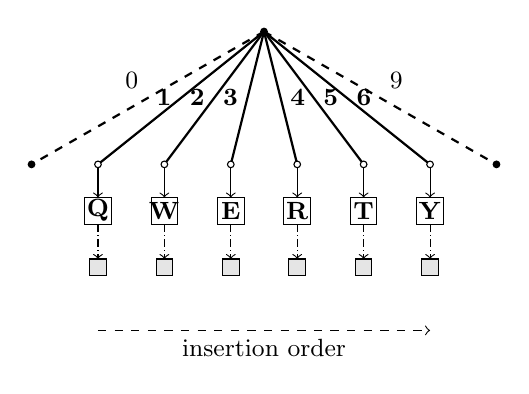
\begin{tikzpicture}[scale=1.2]

  %% node to node
  \small
  \draw[dashed, thick] (0pt,0pt) -- node[anchor=south east]{0} (-70pt,-40pt);
  \draw[thick] (0pt,0pt) -- node[anchor=east]{\textbf{1}} (-50pt,-40pt);
  \draw[thick] (0pt,0pt) -- node[anchor=east]{\textbf{2}} (-30pt,-40pt);
  \draw[thick] (0pt,0pt) -- node[anchor=east]{\textbf{3}} (-10pt,-40pt);
  \draw[thick] (0pt,0pt) -- node[anchor=west]{\textbf{4}} ( 10pt,-40pt);
  \draw[thick] (0pt,0pt) -- node[anchor=west]{\textbf{5}} ( 30pt,-40pt);
  \draw[thick] (0pt,0pt) -- node[anchor=west]{\textbf{6}} ( 50pt,-40pt);
  \draw[dashed, thick] (0pt,0pt) -- node[anchor=south west]{9} ( 70pt,-40pt);

  %% node to element
  \draw[->] (-50pt,-40pt) -- (-50pt,-50pt);
  \draw[->] (-30pt,-40pt) -- (-30pt,-50pt);
  \draw[->] (-10pt,-40pt) -- (-10pt,-50pt);
  \draw[->] ( 10pt,-40pt) -- ( 10pt,-50pt);
  \draw[->] ( 30pt,-40pt) -- ( 30pt,-50pt);
  \draw[->] ( 50pt,-40pt) -- ( 50pt,-50pt);

  %% element to desambiguator
  \draw[->,densely dashdotted] ( -50pt,-58pt) -- ( -50pt,-68.5pt);
  \draw[->,densely dashdotted] ( -30pt,-58pt) -- ( -30pt,-68.5pt);
  \draw[->,densely dashdotted] ( -10pt,-58pt) -- ( -10pt,-68.5pt);
  \draw[->,densely dashdotted] (  10pt,-58pt) -- (  10pt,-68.5pt);
  \draw[->,densely dashdotted] (  30pt,-58pt) -- (  30pt,-68.5pt);
  \draw[->,densely dashdotted] (  50pt,-58pt) -- (  50pt,-68.5pt);

  \draw[fill=black] (  0pt,  0pt) circle (1pt);
  \draw[fill=black] (-70pt,-40pt) circle (1pt);
  \draw[fill=white] (-50pt,-40pt) circle (1pt);
  \draw[fill=white] (-30pt,-40pt) circle (1pt);
  \draw[fill=white] (-10pt,-40pt) circle (1pt);
  \draw[fill=white] ( 10pt,-40pt) circle (1pt);
  \draw[fill=white] ( 30pt,-40pt) circle (1pt);
  \draw[fill=white] ( 50pt,-40pt) circle (1pt);
  \draw[fill=black] ( 70pt,-40pt) circle (1pt);

  %% elements
  \draw[fill=white](-50pt,-54pt)
  node{\textbf{Q}}+(-4pt,-4pt)rectangle+(4pt,4pt) ;
  \draw[fill=white](50pt,-54pt)
  node{\textbf{Y}} +(-4pt,-4pt) rectangle +(4pt,4pt) ;
  \draw[fill=white]( 10pt,-54pt)
  node{\textbf{R}} +(-4pt,-4pt) rectangle +(4pt,4pt) ;
  \draw[fill=white] ( -30pt,-54pt)
  node{\textbf{W}} +(-4pt,-4pt) rectangle +(4pt,4pt) ;
  \draw[fill=white] ( -10pt,-54pt)
  node{\textbf{E}} +(-4pt,-4pt) rectangle +(4pt,4pt) ;
  \draw[fill=white]( 30pt,-54pt)
  node{\textbf{T}} +(-4pt,-4pt) rectangle +(4pt,4pt) ;

  %% desambiguator
  \draw[fill=gray!20] (-50pt,-71pt) +(-2.5pt,-2.5pt) rectangle +(2.5pt,2.5pt);
  \draw[fill=gray!20] (-30pt,-71pt) +(-2.5pt,-2.5pt) rectangle +(2.5pt,2.5pt);
  \draw[fill=gray!20] (-10pt,-71pt) +(-2.5pt,-2.5pt) rectangle +(2.5pt,2.5pt);
  \draw[fill=gray!20] ( 10pt,-71pt) +(-2.5pt,-2.5pt) rectangle +(2.5pt,2.5pt);
  \draw[fill=gray!20] ( 30pt,-71pt) +(-2.5pt,-2.5pt) rectangle +(2.5pt,2.5pt);
  \draw[fill=gray!20] ( 50pt,-71pt) +(-2.5pt,-2.5pt) rectangle +(2.5pt,2.5pt);

  %% insertion order
  \draw[->,dashed] (-50pt, -90pt) -- node[anchor=north]{insertion order}
  (50pt, -90pt);

\end{tikzpicture}
}
  \hspace{50pt}
  \subfloat[Worst case.]
  [Worst case.]
  {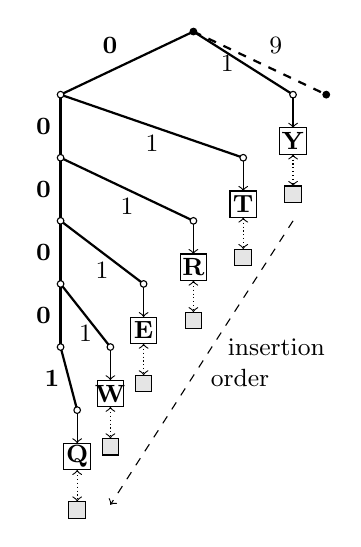
\begin{tikzpicture}[scale=1.2]

\newcommand\Y{-19}
\newcommand\ADDY{-10}

  %% node to node
  \small
  \draw[thick] (0pt,0pt) -- node[anchor=south east]{\textbf{0}} (-40pt,\Y pt);
  \draw[thick] (0pt,0pt) -- node[anchor=east]{1} (30pt, \Y pt); %% Y
  \draw[thick] (-40pt, \Y pt) -- node[anchor=north]{1} (15pt, 2 * \Y pt); %% T
  \draw[thick] (-40pt, \Y pt) -- node[anchor=east]{\textbf{0}} (-40pt, 2 * \Y pt); %% 0
  \draw[thick] (-40pt, 2*\Y pt) -- node[anchor=north]{1} (0pt, 3 * \Y pt); %% R
  \draw[thick] (-40pt, 2*\Y pt)-- node[anchor=east]{\textbf{0}}(-40pt, 3 * \Y pt); %% 0
  \draw[thick] (-40pt, 3*\Y pt) -- node[anchor=north]{1}(-15pt,4 * \Y pt); %% E
  \draw[thick] (-40pt, 3*\Y pt) -- node[anchor=east]{\textbf{0}}(-40pt,4 * \Y pt); %% 0
  \draw[thick] (-40pt, 4*\Y pt) -- node[anchor=north]{1}(-25pt,5 * \Y pt); %% W
  \draw[thick] (-40pt, 4*\Y pt) -- node[anchor=east]{\textbf{0}}(-40pt,5 * \Y pt); %% 0
  \draw[thick] (-40pt, 5*\Y pt) -- node[anchor=east]{\textbf{1}}(-35pt,6 * \Y pt); %% Q

  \draw[dashed, thick] (0pt,0pt) -- node[anchor=south west]{9} (40pt,\Y pt);

  %% node to element
  \draw[->] ( 30pt, \Y pt) -- ( 30pt, \ADDY + \Y pt); %% Y
  \draw[->] ( 15pt, 2* \Y pt) -- ( 15pt, \ADDY + 2 *\Y pt); %% T
  \draw[->] (  0pt, 3 *\Y pt) -- (  0pt, \ADDY + 3 *\Y pt); %% R
  \draw[->] (-15pt, 4 *\Y pt) -- ( -15pt, \ADDY + 4 *\Y pt); %% E
  \draw[->] (-25pt, 5 *\Y pt) -- ( -25pt, \ADDY + 5 *\Y pt); %% W
  \draw[->] (-35pt, 6 *\Y pt) -- ( -35pt, \ADDY + 6 *\Y pt); %% Q

  %% element to desambiguator
  \draw[<->,densely dotted]
  ( 30pt,-8+ \ADDY + \Y pt) -- ( 30pt,2.75*\ADDY+\Y pt); %% Y
  \draw[<->,densely dotted]
  ( 15pt,-8+ \ADDY + 2* \Y pt) -- ( 15pt,2.75*\ADDY+ 2* \Y pt); %% T
  \draw[<->,densely dotted]
  ( 0pt,-8+ \ADDY + 3* \Y pt) -- (  0pt,2.75*\ADDY+ 3* \Y pt); %% R
  \draw[<->,densely dotted]
  ( -15pt,-8+ \ADDY + 4 *\Y pt) -- ( -15pt,2.75*\ADDY+ 4* \Y pt); %% E
  \draw[<->,densely dotted]
  ( -25pt,-8+ \ADDY + 5 *\Y pt) -- ( -25pt,2.75*\ADDY+ 5*\Y pt); %% W
  \draw[<->,densely dotted]
  ( -35pt,-8+ \ADDY + 6* \Y pt) -- ( -35pt,2.75*\ADDY+ 6*\Y pt); %% Q

  %% node
  \draw[fill=black] (0pt,0pt) circle (1pt); %% rooot
  \draw[fill=white] ( 30pt, \Y pt) circle (1pt); %% Y
  \draw[fill=white] (-40pt, \Y pt) circle (1pt); %% 0
  \draw[fill=white] ( 15 pt, 2 * \Y pt) circle (1pt); %% T
  \draw[fill=white] (-40pt, 2 * \Y pt) circle (1pt); %% 0
  \draw[fill=white] (  0 pt, 3 * \Y pt) circle (1pt); %% R
  \draw[fill=white] (-40pt, 3 * \Y pt) circle (1pt); %% 0
  \draw[fill=white] (-15 pt, 4 * \Y pt) circle (1pt); %% E
  \draw[fill=white] (-40pt, 4 * \Y pt) circle (1pt); %% 0
  \draw[fill=white] (-25 pt, 5 * \Y pt) circle (1pt); %% W
  \draw[fill=white] (-40pt, 5 * \Y pt) circle (1pt); %% 0
  \draw[fill=white] (-35 pt, 6 * \Y pt) circle (1pt); %% Q

  \draw[fill=black] ( 40pt, \Y pt) circle (1pt);


  %% elements
  \draw[fill=white] ( 30pt, -4 + \ADDY + \Y pt)
  node{\textbf{Y}} +(-4pt,-4pt) rectangle +(4pt,4pt) ; %% Y
  \draw[fill=white] ( 15pt, -4 + \ADDY +  2 *\Y pt)
  node{\textbf{T}} +(-4pt,-4pt) rectangle +(4pt,4pt) ; %% T
  \draw[fill=white] (  0pt, -4 + \ADDY +  3* \Y pt)
  node{\textbf{R}} +(-4pt,-4pt) rectangle +(4pt,4pt) ; %% R
  \draw[fill=white] (-15pt, -4 + \ADDY + 4 *\Y pt)
  node{\textbf{E}} +(-4pt,-4pt) rectangle +(4pt,4pt) ; %% E
  \draw[fill=white] (-25pt, -4 + \ADDY + 5 * \Y pt)
  node{\textbf{W}} +(-4pt,-4pt) rectangle +(4pt,4pt) ; %% W
  \draw[fill=white] (-35pt, -4 + \ADDY + 6 *\Y pt)
  node{\textbf{Q}} +(-4pt,-4pt) rectangle +(4pt,4pt) ; %% Q

  %% desambiguator
  \draw[fill=gray!20]( 30pt, -2.5 + 2.75 * \ADDY + \Y pt)
  +(-2.5pt,-2.5pt) rectangle +(2.5pt,2.5pt);
  \draw[fill=gray!20]( 15pt, -2.5 + 2.75 * \ADDY +2 *\Y pt)
  +(-2.5pt,-2.5pt) rectangle +(2.5pt,2.5pt);
  \draw[fill=gray!20](  0pt, -2.5 + 2.75 * \ADDY + 3*\Y pt)
  +(-2.5pt,-2.5pt) rectangle +(2.5pt,2.5pt);
  \draw[fill=gray!20](-15pt, -2.5 + 2.75 * \ADDY +4*\Y pt )
  +(-2.5pt,-2.5pt) rectangle +(2.5pt,2.5pt);
  \draw[fill=gray!20](-25pt, -2.5 + 2.75 * \ADDY + 5*\Y pt)
  +(-2.5pt,-2.5pt) rectangle +(2.5pt,2.5pt);
  \draw[fill=gray!20](-35pt, -2.5 + 2.75 * \ADDY +6*\Y pt) 
  +(-2.5pt,-2.5pt) rectangle +(2.5pt,2.5pt);

  %% insertion order
  \draw[->,dashed] (30pt, 3 * \Y pt) -- node[anchor=west,align=left]
  {\ \ insertion\\ order} (-25pt, 7.5 * \Y pt);

\end{tikzpicture}
}
  \caption{\label{fig:allocpathexample} Two trees filled with the resulting
    identifiers of two different permutations resulting in an identical sequence
    QWERTY. They use the same function \textsc{allocPath} which allocates the
    leftmost branch in the tree. All paths of the nearly optimal case have a
    length of 1 while the tree of the worst case grows up to a depth of 6.}
\end{figure*}

Figure~\ref{fig:allocpathexample} illustrates the difficulties of designing a
function allocating paths. It represents the underlying trees of two sequences
using the allocation function that allocates the leftmost branch available at
the lowest depth possible. In both cases the final sequence is QWERTY. However,
the insertion order of characters is different. In the first case, Q is inserted
first at position 0, followed by W at position 1 (after Q) then E is inserted at
position 3 (after W), etc. We call the sequence of insert operations
$[(\text{Q},\,0)$, $(\text{W},\,1)$, $(\text{E},\,2)$, $\ldots]$ the
\emph{editing sequence}. In the second case, Character Y is inserted first at
position 0 as the sequence is initially empty. Then T is inserted. However as
the final intended word is QWERTY, T has to be inserted at a position before Y
that represents the current state of the sequence. T is thus inserted at
position 0 shifting Character Y to position 1, etc. The editing sequence that
corresponds to this case is $[(\text{Y},\,0)$, $(\text{T},\,0)$,
$(\text{R},\,0)$, $\ldots]$.


\begin{itemize}
\item Case 1: Since Function \textsc{allocPath} allocates the leftmost branches,
  the following editing sequence $[(\text{Q},\,0)$, $(\text{W},\,1)$,
  $(\text{E},\,2)$, $\ldots]$ leads to the paths
  $\langle [1],\, \text{Q}\rangle$, $\langle [2],\, \text{W}\rangle$,
  $\langle [3],\, \text{E}\rangle$, etc. In this case, the depth of the tree
  never grows. In this regard, the strategy of \textsc{allocPath} is very
  efficient in terms of the size of the allocated identifiers.

\item Case 2: The editing sequence $[(\text{Y},\,0)$, $(\text{T},\,0)$,
  $(\text{R},\,0)$, $\ldots]$ leads to an increase of the tree depth per
  insertion. Indeed, as an element gets the smallest value at its level, there
  is no room for a new element at the same level, hence a new level. The
  resulting sequence is $\langle [1],\, \text{}Y\rangle$,
  $\langle [0.1],\, \text{T}\rangle$, $\langle [0.0.1],\, \text{R} \rangle$,
  etc. Consequently, the paths grow very fast.
\end{itemize}

This example shows how the insertion order impacts the length of the allocated
paths. Unfortunately, the insertion order cannot be predicted, nor the size of
the final sequence. Prior work on sequences often made the assumption of a
left-to-right editing due to observations made on
corpus~\cite{preguica2009commutative, weiss2009logoot}. However, there exist
human edited documents that do not correspond to this kind of
editing~\cite{nedelec2013lseq}.
%% Indeed, the editing depends on the type of the document and to the activity
%% for example when correcting a document the editing in mainly random as the
%% insertions and deletions corresponds to errors distributed in the document.
We are looking for an allocation function which provides identifiers with a
sublinear space complexity compared to the number of insertions whatever the
editing sequence. Such allocation function would avoid the need for consensus
algorithm~\cite{mostefaoui2015signature} and would make CRDT-based editors a
practicable alternative to the current mainstream editors.
 
%%% Local Variables:
%%% mode: latex
%%% TeX-master: "../paper"
%%% End:
